\documentclass{article}
\usepackage{epcc}
\usepackage{hyperref}
\usepackage{listings}

\hyphenpenalty=500

\title{Domain Decomposition: Computational Fluid Dynamics}

\begin{document}

\makeEPCCtitle

\section{Introduction and Aims} 

This exercise takes an example from one of the most common
applications of HPC resources: Fluid Dynamics. We will look at how a
simple fluid dynamics problem can be run on a system like ARCHER and
how varying the number of processes it runs on and the problem size
affect the performance of the code. This will require a set of
simulations to be run and performance metrics to be recorded and
plotted on a graph.

The CFD program differs from the more straightforward task farm in
that the problem requires more than source-worker-sink
communications. Here the workers are in regular communication
throughout the calculation.

This exercise aims to introduce:
\begin{itemize}
\item Grids
\item Communications -- Halos
\item Performance metrics
\end{itemize}

\section{Fluid Dynamics}

Fluid Dynamics is the study of the mechanics of fluid flow, liquids
and gases in motion. This encompasses aero-~and hydrodynamics. 
It has wide ranging applications, from theoretical studies of flow to
engineering problems such as vessel and structure design, and 
plays an important role in weather modelling. Simulating and solving
fluid dynamic problems requires large computational resources.

Fluid dynamics is an example of continuous system which can be
described by Partial Differential Equations. For a computer to
simulate these systems, the equations must be discretised onto a
grid. If this grid is regular, then a finite difference approach can
be used. Using this method means that the value at any point in the
grid is updated using some combination of the neighbouring points.

\textbf{Discretisation} is the process of approximating a continuous
(i.e. infinite-dimensional) problem by a finite-dimensional problem
suitable for a computer. This is often accomplished by putting the
calculations into a grid or similar construct.

\subsection{The Problem}

In this exercise the finite difference approach is used to determine
the flow pattern of a fluid in a cavity. For simplicity, the liquid is
assumed to have zero viscosity which implies that there can be no
vortices (i.e. no whirlpools) in the flow. The cavity is a square box
with an inlet on one side and an outlet on another as shown below.
 
\begin{figure}[th] %  figure placement: here, top, bottom, or page
{\centerline{\resizebox{0.60\hsize}{-0.60\hsize}{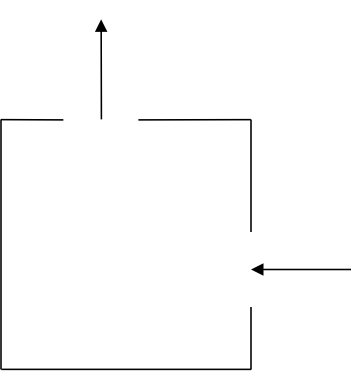
\includegraphics{box.png}}}}
   \caption{The Cavity}
   \label{fig:box}
\end{figure}

\subsection{Mathematical formulation and the Jacobi algorithm solution}
In two dimensions it is easiest to work with the {\em stream function}
$\Psi$ (see below for how this relates to the fluid velocity). For
zero viscosity $\Psi$ satisfies the following equation:

\[
\nabla^2\Psi = \frac{\partial^2 \Psi}{\partial x^2} + \frac{\partial^2 \Psi}{\partial y^2} = 0
\]

The finite difference version of this equation is: 

\[ \Psi_{i-1,j} + \Psi_{i+1,j} + \Psi_{i,j-1} + \Psi_{i,j+1} - 4\Psi_{i,j} = 0 \]


With the boundary values fixed, the stream function can be calculated
for each point in the grid by averaging the value at that point with
its four nearest neighbours. The process continues until the algorithm
converges on a solution which stays unchanged by the averaging
process. This simple approach to solving a PDE is called the Jacobi
Algorithm.

In order to obtain the flow pattern of the fluid in the cavity we want
to compute the velocity field $\tilde{u}$. The $x$ and $y$ components
of $\tilde{u}$ are related to the stream function by

\[ u_x =   \frac{\partial \Psi}{\partial y} = \frac{1}{2}(\Psi_{i,j+1} - \Psi_{i,j-1}) \]
\[ u_y = - \frac{\partial \Psi}{\partial x} = - \frac{1}{2}(\Psi_{i+1,j} - \Psi_{i-1,j}) \]

This means that the velocity of the fluid at each grid point can also
be calculated from the surrounding grid points.  




\subsection{Pseudocode for the Jacobi algorithm}
The outline of the algorithm for calculating the velocities is as follows: \\

\verb+   Set the boundary values for +$\Psi$ \verb+and+ $\tilde{u}$ \\
\verb+   while (convergence= FALSE) do +\\
\verb+      for each interior grid point do +\\
\verb+         update value of +$\Psi$ \verb+ by averaging with its 4 nearest neighbours +\\
\verb+      end do +\\
\verb+      check for convergence  +\\
\verb+   end do +\\
\verb+   for each interior grid point do +\\
\verb+      calculate+ $u_x$ \\
\verb+      calculate+ $u_y$ \\
\verb+   end do+

For simplicity, here we simply run the calculation for a fixed number
of iterations; a real simulation would continue until some chosen
accuracy was achieved.



\subsection{Breaking up the problem to solve it in parallel}

The calculation of the velocity of the fluid as it flows through the cavity proceeds in two stages: 

\begin{itemize}
\item Calculate the stream function $\Psi$. 
\item Use this to calculate the $x$ and $y$ components of the velocity. 
\end {itemize}

Both of these stages involve calculating the value at each grid point
by combining it with the value of its four nearest neighbours. Thus
the same amount of work is involved in calculating each grid point,
making it ideal for the regular \textbf{domain decomposition}
approach. Figure~\ref{fig:griddy} shows how a two-dimensional grid 
can be broken up into smaller grids to be handled by individual 
processes.

\begin{figure}[ht] %  figure placement: here, top, bottom, or page
{\centerline{\resizebox{0.65\hsize}{!}{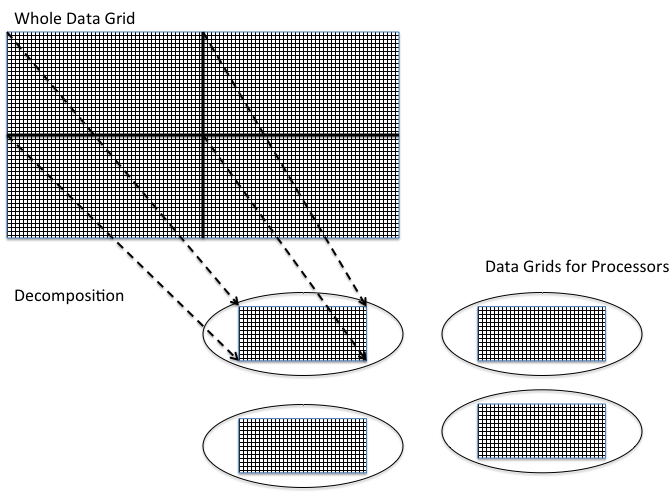
\includegraphics{griddy.png}}}}
   \caption{Breaking up the problem through domain decomposition}
   \label{fig:griddy}
\end{figure}

This approach can be generalised to include cases where slices or
irregular subsections of grids are sent to individual processes and
the results are collated at the end of a calculation cycle.

\subsection{Communicating through Halo swaps}
\begin{figure}[th] %  figure placement: here, top, bottom, or page
{\centerline{\resizebox{0.60\hsize}{!}{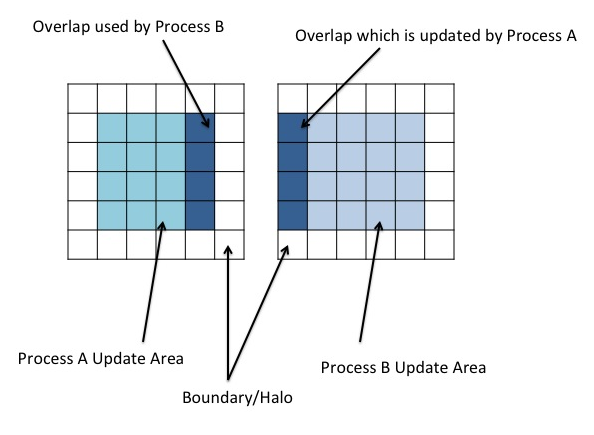
\includegraphics{bound.png}}}}
   \caption{Halo: Process A and Process B}
   \label{fig:bound}
\end{figure}

Splitting the grid into smaller grids introduces a problem computating
values at points on the edges of subgrids, as this requires the values
of neighbouring points, which are part of a neighbouring subgrid whose
values are being computed by a different process. This means that some
form of communication between processes is needed.

One way to tackle this problem is to add a boundary layer to each edge
of each subgrid that adjoins another subgrid. These boundary layers
are not updated by the local process updating the interior points of
the subgrid, but instead by the process working on the neighbouring
subgrid. The boundary layer in the neighbouring subgrid is in turn
updated by the local process. These boundary layers are generally
known as {\em halos}. An example of this is show in Figure
\ref{fig:bound}.

In order to keep the halos up to date, a halo swap must be carried
out. When an element in process B which adjoins the boundary layer
with process A is updated and process A has been updating, the halo
must be swapped to ensure process B uses accurate data. This means
that a communication between processes must take place in order to
swap the boundary data.  This halo swap introduces communications
which, if the grid is split into too many processes or the size of
data transfers is very large, can begin to dominate the runtime
instead of actual processing work. Part of this exercise is to look at
how the number of processes affects the runtime for given problem
sizes, and evaluate what this means for speed up and efficiency.

\subsection{One-dimensional Domain decomposition for CFD example}

In the parallel version of the code provided for this exercise (F-MPI)
we have only decomposed the problem in one dimension, namely the
y-dimension. This means that the problem is sliced up into a series of
rectangular strips. Although for a real problem the domain would
probably be split up in both dimensions as in Figure~\ref{fig:griddy},
splitting across a single dimension makes programming and
understanding the code significantly easier. Each process only needs
to communicate with a maximum of two neighbours, swapping halo data up
and down.

\newpage

\section{Exercises}

\subsection{Compilation}

Use \verb+wget+ to copy the file \verb+cfd.tar.gz+ from the ARCHER web
page for the course to your personal directory on \verb+/work/+ on
ARCHER, as you did for the previous exercises. Now unpack the file and
compile the Fortran code provided for the CFD example as described
below. We have provided a serial version of the code (directory F-SER)
as well as a parallel version of the code using the domain
decomposition approach and MPI for halo swap communications as
described above (directory F-MPI). After compilation an executable
file called \textbf{cfd} will have been created in each case.

\begin{lstlisting}[frame=single]
  guestXX@archer:~> tar -zxvf cfd.tar.gz 
  cfd/
  cfd/F-MPI/
  cfd/F-SER/
  cfd/F-SER/boundary.f90
  cfd/F-SER/cfd.f90
  cfd/F-SER/cfd.pbs
  cfd/F-SER/cfdio.f90
  cfd/F-SER/jacobi.f90
  cfd/F-SER/Makefile
  cfd/F-MPI/boundary.f90
  cfd/F-MPI/cfd.f90
  cfd/F-MPI/cfd.pbs
  cfd/F-MPI/cfdio.f90
  cfd/F-MPI/jacobi.f90
  cfd/F-MPI/Makefile
  guestXX@archer:~> cd cfd/F-SER
  guestXX@archer:~/cfd/F-SER> make
  ftn -g -c boundary.f90
  ftn -g -c jacobi.f90
  ftn -g -c cfdio.f90
  ftn -g -c cfd.f90
  ftn -g -o cfd boundary.o cfd.o cfdio.o jacobi.o 
  guestXX@archer:~/cfd/F-SER> cd ./../F-MPI
  guestXX@archer:~/cfd/F-MPI> make
  ftn -g -c boundary.f90
  ftn -g -c jacobi.f90
  ftn -g -c cfdio.f90
  ftn -g -c cfd.f90
  ftn -g -o cfd boundary.o cfd.o cfdio.o jacobi.o 
\end{lstlisting}

\subsection{Run the program}

\subsubsection{Running in serial}
As long as you do not run for longer than a minute, say, 
you can execute the serial executable on the login
node directly from the command line as follows:

\begin{lstlisting}[frame=single]
guestXX@archer:~/cfd/F-SER> ./cfd <scale> <numiter>
\end{lstlisting}

where you should replace \verb+<scale>+ and \verb+<numiter>+
by integers that have the following meaning:

\begin{itemize}
\item{\bf <scale>}: a scale factor that is used to set the size of the
  grid (see below)
\item{\bf <numiter>}: how many iterations to run the Jacobi algorithm for.
\end{itemize}

The mimimum problem size (scale factor = 1) is taken as a
$32 \times 32$ grid. The actual problem size can be chosen by scaling
this basic size, for example with a scale factor of 4 then it will use
a $128 \times 128$ grid.

After the executable has finished running the output on screen 
should look something like this (depending on the exact parameters):

\begin{lstlisting}[frame=single]
 ./cfd 4 5000
 Scale factor =   4, iterations =   5000
 Irrotational flow
 Running CFD on  128 x  128 grid in serial 

 Starting main loop ...

 completed iteration         1000
 completed iteration         2000
 completed iteration         3000
 completed iteration         4000
 completed iteration         5000

 ... finished

 After      5000 iterations, error is  0.1872E-03
 Time for   5000 iterations was  0.3136     seconds
 Each individual iteration took  0.6273E-04 seconds

 Writing output file ...
  ... finished

 CFD completed
\end{lstlisting}

The code also produces some graphical output in the form of a gnuplot
file \verb+cfd.plt+. Provided you have logged in to ARCHER with X11
forwarding turned on (\verb+ssh -X+ from the command line) you can
view this as follows:

\begin{lstlisting}[frame=single]
  guestXX@archer:~> gnuplot -persist cfd.plt
\end{lstlisting}

which should produce a picture similar to Figure~\ref{fig:out}. 

\begin{figure}[ht] %  figure placement: here, top, bottom, or page
   \centering
{\centerline{\includegraphics{output.pdf}}}
   \caption{Output Image}
   \label{fig:out}
\end{figure}

\newpage

If the fluid is flowing down the right-hand edge then along the
bottom, rather than through the middle of the cavity, then this is an
indication that the Jacobi algorithm has not yet converged. 
Convergence requires more iterations on larger problem sizes.



\subsubsection{Running in parallel}
Use emacs or your preferred editor to look at the \verb+cfd.pbs+ batch
script inside the \verb+F-MPI+ directory:
\begin{lstlisting}[frame=single]
#!/bin/bash --login

#PBS -l select=1
#PBS -l walltime=00:05:00
#PBS -A y14
#PBS -N cfd

#Change to directory that the job was submitted from
cd $PBS_O_WORKDIR

aprun -n 4 ./cfd 4 5000
\end{lstlisting}
The argument to aprun has the following meaning:
\begin{itemize}
\item{\bf -n 4}: run the code on 4 processes;
\end{itemize}
The arguments to cfd are the same as in the serial case, with the 
scale factor now setting the size of the overall grid (which will be
decomposed into smaller subgrids). Varying the number of processes
and scale factor allows us to investigate Amdahl's and Gustafson's
laws. The number of iterations is not particularly important as we are
interested in the time per iteration. You can increase the number of
iterations to ensure that the code does not run too fast on large
numbers of processes, or decrease it so it is not too slow for large
problem sizes. Two things to note:

\begin{itemize}

\item The code assumes the problem size decomposes exactly onto the
  process grid. If this is not the case (e.g. scale factor = 2 with 7
  processes, since 7 is not a divisor of 64) it will complain and
  exit.

\item Again if the output picture looks strange then you may not have used a
  sufficient number of iterations to converge to the solution. This is
  not a problem in terms of the performance figures, but it is worth
  running with more iterations just to check that the code is
  functioning correctly
\end{itemize}

Once you have run the job via the PBS batch system, the output file
should look something like this (depending on the exact parameters):

\begin{lstlisting}[frame=single]
 Scale factor =   4, iterations =   5000
 Irrotational flow
 Running CFD on  128 x  128 grid using    4 process(es)
 
 Starting main loop ...
 
 completed iteration  1000
 completed iteration  2000
 completed iteration  3000
 completed iteration  4000
 completed iteration  5000
 
 ... finished
 
 After      5000 iterations, error is  0.1872E-03
 Time for   5000 iterations was  0.1763     seconds
 Each individual iteration took  0.3527E-04 seconds
 
 Writing output file ...
  ... finished
 
 CFD completed
\end{lstlisting}



\subsection{Performance Evaluation}
The next part of this exercise will be to determine what the best
configuration for a group of problems sizes in the CFD code would
be. This will be worked out using two measures: speed-up and
efficiency.

\subsubsection{Speedup}
The speedup of a parallel code is how much faster the parallel version
runs compared to a non-parallel version. Taking the time to run the
code on 1 process is $T_1$ and to run the code on $P$ processes is
$T_P$, the speed-up $S$ is found by:
\begin{equation}
S = \frac{T_1}{T_P}
\end{equation}

\subsubsection{Efficiency}

Efficiency is how the well the resources (available processing power in
this case) are being used. This can be thought of as the speed-up (or
slow-down) per process. Efficiency $E$ can be defined as:
\begin{equation}
E = \frac{S}{P} =  \frac{T_1}{P T_P}
\end{equation}

where $E = 1.0$ means 100\% efficiency, i.e. perfect scaling.

\subsubsection{Doing The Work}

The two main evaluation points:
\begin{itemize}

\item How do the speed-up and efficiency of the program vary as the
  number of processes is increased?

\item Does this change as the problem size is varied? 

\end{itemize}

To investigate the speed-up and parallel efficiency the code should be
run using the same problem size but with varying numbers of
processes. Calculate the speed-up and efficiency (tables are provided
overleaf for this) and plot a graph of the speed-up against the number
of processes. Is there any apparent pattern, e.g. does it follow
Amdahl's law?

Now choose a different problem size and repeat the exercise. To
increase the problem size increase the scale factor; to decrease the
size, decrease the scale factor. For example, setting \textbf{scale
  factor} = 2 will give a problem size of 64x64; \textbf{scale factor}
= 6 gives a size of 192x192.

What is the effect of problem size the parallel scaling of the code?

Note that, for large numbers of processes, you may have to increase
the number of iterations so that the code runs for a reasonable length
of time -- it is difficult to interpet timings quantitatively if a
program runs too quickly, e.g. for much less than a second. The time
per iteration, however, should be independent of the number of
iterations.

\newpage

1. problem size (scalefactor) = \underline{\hspace{3cm}} iterations =\underline{\hspace{3cm}}

\begin{center}
\begin{tabular}{|c||c|c|c|}
\hline
No of processes & Time per iteration & Speed-Up & Efficiency \\
\hline
\hline
1 & & & \\
\hline
2 & & & \\
\hline
4 & & & \\
\hline
8 & & & \\
\hline
16 & & & \\
\hline
32 & & & \\
\hline
64 & & & \\
\hline
128 & & & \\
\hline
\end{tabular}
\end{center}

2. problem size (scalefactor) = \underline{\hspace{3cm}} iterations =\underline{\hspace{3cm}}

\begin{center}
\begin{tabular}{|c||c|c|c|}
\hline
No of processes & Time per iteration & Speed-Up & Efficiency \\
\hline
\hline
1 & & & \\
\hline
2 & & & \\
\hline
4 & & & \\
\hline
8 & & & \\
\hline
16 & & & \\
\hline
32 & & & \\
\hline
64 & & & \\
\hline
128 & & & \\
\hline
\end{tabular}
\end{center}

3. problem size (scalefactor) = \underline{\hspace{3cm}} iterations =\underline{\hspace{3cm}}

\begin{center}
\begin{tabular}{|c||c|c|c|}
\hline
No of processes & Time per iteration & Speed-up & Efficiency \\
\hline
\hline
1 & & & \\
\hline
2 & & & \\
\hline
4 & & & \\
\hline
8 & & & \\
\hline
16 & & & \\
\hline
32 & & & \\
\hline
64 & & & \\
\hline
128 & & & \\
\hline
\end{tabular}
\end{center}

4. problem size (scalefactor) = \underline{\hspace{3cm}} iterations =\underline{\hspace{3cm}}

\begin{center}
\begin{tabular}{|c||c|c|c|}
\hline
No of processes & Time per iteration & Speed-up & Efficiency \\
\hline
\hline
1 & & & \\
\hline
2 & & & \\
\hline
4 & & & \\
\hline
8 & & & \\
\hline
16 & & & \\
\hline
32 & & & \\
\hline
64 & & & \\
\hline
128 & & & \\
\hline
\end{tabular}
\end{center}

\newpage

\section{Compiler Investigation}

We will use the CFD example to investigate how different compilers and
options affect performance.

\subsection{Changing compilers on ARCHER}

On ARCHER, the Fortran compiler is always called \verb+ftn+. However,
what compiler this actually points to is determined by what module you
have loaded.
For example, to switch from the default (Cray) compiler to the Intel
compiler.


\begin{verbatim}
  guestXX@archer:~> module switch PrgEnv-cray PrgEnv-intel
  guestXX@archer:~> make clean
  guestXX@archer:~> make
\end{verbatim}

Here. \verb+make clean+ ensures that all compiled code is removed
which means that the new code will be built with the new
compiler. Note that this also removes output files velocity.dat,
colourmap.dat, and cfd.plt, so if you wish to keep these you should
rename them.  The GNU compiler module is called
\verb+PrgEnv-gnu+.

\subsection{Exercises}

Here are a number of suggestions:

\begin{itemize}

\item By default, the code is built with the \verb+-g+ debugging
  option. Edit the Makefile to remove this and recompile - what is the
  effect on performance?

\item What is the difference between the performance of the code using
  the three different compilers (Cray, Intel and GNU) with no compiler
  options?

\item It is not really fair to compare compiler performance using
  default options: one compiler may simply have higher default
  settings than another. Using the option suggested in ``Useful compiler options'' at \href{http://www.archer.ac.uk/documentation/user-guide/development.php}{http://www.archer.ac.uk/documentation/user-guide/development.php}, compare the best performance you can get with each compiler.

\item The code can actually simulate fluids with a finite
  viscosity. You can pass a third parameter to the program, the
  Reynolds Number$ Re$, which here is effectively the input velocity of
  the fluid. For example, \verb+aprun -n 4 ./cfd 4 5000 1.8+ sets $Re
  = 1.8$ (note that the code becomes unstable for values of $Re >
  3.7$).  This increases the computation required so the code will be
  slower, although the actual amount of computation is independent of
  the value of $Re$.

  Investigate the parallel scaling behaviour of the code for some
  particular value of $Re$. Is it any different from the previous
  (zero viscosity) case?

\begin{figure}[bh] %  figure placement: here, top, bottom, or page
   \centering
{\centerline{\resizebox{0.55\hsize}{!}{\includegraphics{outputre.pdf}}}}
   \caption{Simulation with $Re = 1.8$}
   \label{fig:outre}
\end{figure}

\end{itemize}

\end{document}
